% ============================================================
% Axonal-BGP: Agent-Signed Inter-Domain Routing on the
% ECCA Substrate
%
% A companion paper to ECCA v3.0
%
% Compile: pdflatex main.tex && bibtex main && pdflatex main.tex && pdflatex main.tex
% ============================================================

\documentclass[11pt,twocolumn]{article}

% ---- Packages ----
\usepackage[utf8]{inputenc}
\usepackage[T1]{fontenc}
\usepackage{lmodern}
\usepackage{microtype}
\usepackage[margin=2cm,top=2.5cm,bottom=2.5cm]{geometry}
\usepackage{amsmath,amssymb,amsthm}
\usepackage{algorithm}
\usepackage{algpseudocode}
\usepackage{graphicx}
\usepackage{tikz}
\usetikzlibrary{arrows.meta,positioning,shapes.geometric,fit,calc,decorations.pathreplacing,backgrounds}
\usepackage{booktabs}
\usepackage{multirow}
\usepackage{enumitem}
\usepackage{xcolor}
\usepackage{hyperref}
\usepackage{cleveref}
\crefname{listing}{Listing}{Listings}
\Crefname{listing}{Listing}{Listings}
\crefname{lstlisting}{Listing}{Listings}
\Crefname{lstlisting}{Listing}{Listings}
\usepackage{caption}
\usepackage{subcaption}
\usepackage{listings}
\usepackage{float}
\usepackage{mathtools}
\usepackage{thmtools}
\usepackage{fancyhdr}
\usepackage{titlesec}
\usepackage{balance}

% ---- Color Definitions ----
\definecolor{eccacyan}{HTML}{0097A7}
\definecolor{eccamagenta}{HTML}{AB47BC}
\definecolor{eccagreen}{HTML}{2E7D32}
\definecolor{eccacode}{HTML}{F5F5F5}
\definecolor{eccadark}{HTML}{263238}
\definecolor{eccablue}{HTML}{1565C0}
\definecolor{eccaorange}{HTML}{E65100}

% ---- Hyperref Config ----
\hypersetup{
  colorlinks=true,
  linkcolor=eccablue,
  citecolor=eccacyan,
  urlcolor=eccamagenta,
  pdftitle={Axonal-BGP: Agent-Signed Inter-Domain Routing on the ECCA Substrate},
  pdfauthor={},
  pdfsubject={Inter-domain routing security},
  pdfkeywords={BGP, RPKI, BGPsec, agent-signed routing, blockchain oracle, residue economics, human-in-the-loop, kill switch}
}

% ---- Listings Config (Solidity-flavoured) ----
\lstdefinelanguage{solidity}{
  morekeywords={contract,abstract,interface,function,external,internal,public,private,view,pure,payable,returns,return,if,else,for,while,emit,event,struct,mapping,address,uint,uint8,uint256,int,bool,bytes,bytes32,string,memory,calldata,storage,require,modifier,constructor,onlyOwner,immutable,constant,is,using,enum,true,false,this,new,override,virtual,indexed},
  morecomment=[l]{//},
  morecomment=[s]{/*}{*/},
  morestring=[b]"
}
\lstset{
  basicstyle=\ttfamily\scriptsize,
  backgroundcolor=\color{eccacode},
  frame=single,
  rulecolor=\color{gray!30},
  breaklines=true,
  captionpos=b,
  numbers=left,
  numberstyle=\tiny\color{gray},
  keywordstyle=\color{eccablue}\bfseries,
  commentstyle=\color{eccagreen}\itshape,
  stringstyle=\color{eccamagenta},
  showstringspaces=false,
  tabsize=2,
  language=solidity
}

% ---- Theorem Environments ----
\theoremstyle{definition}
\newtheorem{definition}{Definition}[section]
\newtheorem{property}{Property}[section]
\theoremstyle{plain}
\newtheorem{theorem}{Theorem}[section]
\newtheorem{lemma}[theorem]{Lemma}
\newtheorem{corollary}[theorem]{Corollary}
\newtheorem{proposition}[theorem]{Proposition}
\theoremstyle{remark}
\newtheorem{remark}{Remark}[section]

% ---- Section Formatting ----
\titleformat{\section}{\large\bfseries\sffamily}{\thesection}{1em}{}
\titleformat{\subsection}{\normalsize\bfseries\sffamily}{\thesubsection}{1em}{}
\titleformat{\subsubsection}{\normalsize\itshape\sffamily}{\thesubsubsection}{1em}{}

% ---- Headers ----
\pagestyle{fancy}
\fancyhf{}
\fancyhead[L]{\small\sffamily Axonal-BGP: Agent-Signed Inter-Domain Routing}
\fancyhead[R]{\small\sffamily\thepage}
\renewcommand{\headrulewidth}{0.4pt}

% ---- Custom Commands ----
\newcommand{\ecca}{\textsc{Ecca}}
\newcommand{\axonal}{\textsc{Axonal-BGP}}
\newcommand{\stack}{\textsc{Stack}}
\newcommand{\sleeve}{\textsc{Sleeve}}
\newcommand{\contractname}[1]{\textsc{#1}}
\newcommand{\code}[1]{\texttt{#1}}
\newcommand{\R}{\mathbb{R}}
\newcommand{\N}{\mathbb{N}}
\DeclareMathOperator{\merkleroot}{MerkleRoot}
\DeclareMathOperator{\shatwofiftysix}{SHA256}

% ============================================================
\begin{document}

% ---- Title ----
\twocolumn[
\begin{center}
  {\LARGE\bfseries\sffamily \axonal{}: Agent-Signed Inter-Domain Routing on the ECCA Substrate}\par\vspace{0.4em}
  {\large\sffamily A Token-Bounded Routing Protocol with Residue-Funded Convergence and Oracle-Mediated Human Veto}\par\vspace{1.5em}
  {\normalsize\sffamily RNG}\par\vspace{0.3em}
  {\small\ttfamily rng@infrasim.org}\par\vspace{1.5em}
  {\normalsize
    \textit{Working Paper --- Preprint}\par\vspace{0.3em}
    Draft Version 0.1 \quad$\cdot$\quad May 2026
  }\par\vspace{2em}
\end{center}

\begin{center}
\parbox{0.92\textwidth}{
\textbf{\sffamily Abstract} ---
Border Gateway Protocol (BGP) remains the de-facto inter-domain routing protocol of the public Internet, yet a quarter-century of deployment experience has shown it to be structurally vulnerable to prefix hijacks, route leaks, and origin misconfigurations. Cryptographic overlays such as RPKI~\cite{rfc6480} and BGPsec~\cite{rfc8205} have addressed origin authentication and (partially) path validation, but they assume static trust roots, no economic feedback, and no in-band mechanism for incident response. We present \axonal{}, an experimental routing protocol layered on the \ecca{} distributed-cognition substrate~\cite{ecca2026}. Routing decisions are emitted by autonomous \emph{router agents}, each anchored to an on-chain \code{StackIdentity} NFT, signed with the agent's ed25519 key, and committed every 4-second epoch into the Medulla proof-of-work chain via the same Coherence Root mechanism that \ecca{} uses for memory and inference workloads. Misbehaviour---bogus origins, leaked AS-paths, MOAS conflicts, route flaps---is materialised as \emph{routing-residue} objects, identical in structure to the residues that fund self-healing in \ecca{}'s memory layer. We introduce two new smart contracts: a \contractname{ResidueToRoutingSwap} that lets resolvers convert earned ResidueToken into RoutingToken at an Epoch-Binding-Curve-protected rate, funding the bandwidth needed to propagate corrective announcements; and a \contractname{RouteOracle} that observes the swap and the underlying signed-route table and exposes a \code{pause(agentId)} capability gated by a configurable $M$-of-$N$ human-operator multisig. The result is a routing protocol with cryptographic per-route signatures, an economic incentive loop for misbehaviour detection, and a human-in-the-loop emergency stop that does not require BGP-level coordination across operators. We describe the contract design, the protocol wire format, the router-agent service architecture, and a reproducible Kubernetes/k3d demonstration that mirrors the topology of the existing Playfair test.
}
\end{center}
\vspace{1.5em}

\noindent\textbf{\sffamily Keywords:} BGP, inter-domain routing, RPKI, BGPsec, agent-signed routes, blockchain oracles, residue economics, human-in-the-loop, kill-switch governance.
\vspace{2em}
]

% ============================================================
\section{Introduction}\label{sec:intro}
% ============================================================

The Internet's routing fabric is held together by trust. A handful of Tier-1 operators, several thousand Tier-2 transits, and tens of thousands of stub ASes exchange roughly $1.1 \times 10^{6}$ IPv4 prefixes and $2.2 \times 10^{5}$ IPv6 prefixes via BGP-4~\cite{rfc4271}. Every announcement is, in principle, \emph{unauthenticated}: the receiving router has no in-protocol way to verify that the announcer is entitled to originate the prefix or that the AS-path it advertises is the one packets will actually traverse. Two decades of incidents---Pakistan/YouTube (2008), Indosat (2014), Cloudflare/AWS (2022), Rostelecom (multiple)---have demonstrated the operational cost of this trust model.

The IETF's response, the Resource Public Key Infrastructure (RPKI)~\cite{rfc6480} and BGPsec~\cite{rfc8205}, adds cryptographic proofs of origin and path. Adoption has been gradual: as of 2026 roughly half of IPv4 prefixes carry a valid Route Origin Authorisation (ROA), but BGPsec---which requires every AS along a path to sign---remains marginally deployed because the \emph{incentives} are misaligned. Operators bear the signing cost; benefits accrue to receivers downstream. There is no in-band economic feedback.

This paper asks: \emph{what if every routing decision were signed by an autonomous agent whose identity is a tradeable on-chain object, whose memory and reputation persist across epochs, and whose mistakes are economically costly---and whose corrective announcements are economically rewarded?} That question maps almost directly onto the architecture of \ecca{}~\cite{ecca2026}, which already provides:

\begin{enumerate}[leftmargin=*,itemsep=2pt]
  \item Portable cryptographic identity via \code{StackIdentity} ERC-721 tokens with embedded ed25519 pubkeys.
  \item Atomic cross-shard finality via 4-second Coherence Roots committed by the Medulla PoW chain.
  \item A residue economy in which detected misbehaviour (``residues'') becomes a tradeable bounty resolved by the first valid proof.
  \item A bandwidth token (RoutingToken) that gates the right to propagate cross-region state.
\end{enumerate}

\Cref{sec:related} reviews related work. \Cref{sec:protocol} specifies the \axonal{} wire format and the router-agent service. \Cref{sec:contracts} introduces the two new smart contracts. \Cref{sec:residues} catalogues the routing-specific residues. \Cref{sec:hitl} explains the human-in-the-loop pause mechanism. \Cref{sec:experiment} describes the experimental demonstration. \Cref{sec:discussion} discusses limitations and threat model. \Cref{sec:conclusion} concludes.

\subsection{Contributions}

\begin{itemize}[leftmargin=*,itemsep=2pt]
  \item A wire-compatible BGP UPDATE encapsulation in which every advertisement carries an ed25519 signature over $(\mathit{prefix}, \mathit{originAs}, \mathit{asPath}, \mathit{agentTokenId}, \mathit{epoch})$, verifiable in $O(1)$ against the on-chain \code{StackIdentity} registry.
  \item The \contractname{ResidueToRoutingSwap} contract: a one-way conversion path from ResidueToken (earned by detecting misbehaviour) to RoutingToken (needed to propagate withdrawals), priced by an Epoch Binding Curve to dampen flash-conversion attacks.
  \item The \contractname{RouteOracle} contract: an off-chain observer that subscribes to swap events and signed-route commitments, exposes a \code{pause(agentTokenId)} capability gated by a configurable $M$-of-$N$ human-operator multisig, and enforces a hard ceiling on routing emissions when human approval lapses.
  \item A reproducible Kubernetes demonstration with three simulated ASes, four router agents, two scripted hijack scenarios, and a per-epoch fairness audit identical to the existing Playfair test.
\end{itemize}

% ============================================================
\section{Related Work}\label{sec:related}
% ============================================================

\subsection{Inter-domain routing security}

RPKI~\cite{rfc6480,rfc6810} anchors trust at the IANA level, with the five RIRs as Trust Anchors. Validators (Routinator, FORT, OctoRPKI) translate ROAs into VRPs (Validated ROA Payloads) consumed by routers via RTR. RPKI authenticates origin only; it does not protect AS-paths. BGPsec~\cite{rfc8205} adds per-hop signatures over the AS-path but suffers from cubic key-distribution cost and unbounded signature growth on long paths, which has limited deployment. ASPA~\cite{aspa2024} proposes lighter customer/provider relationship attestations. AS-Cones~\cite{snijders24} and Path-End Validation~\cite{cohen18} occupy similar design space. None of these systems treat routing decisions as \emph{agent-issued cryptographic objects} nor offer economic feedback for resolution.

\subsection{Blockchain-based routing experiments}

Earlier proposals---BlockJack~\cite{hari18}, DISCO~\cite{sermpezis20}, and a series of ``BGP on a blockchain'' Master's theses---have experimented with placing the entire routing table on a public ledger. They suffer from throughput limits (BGP processes ${\sim}10^{5}$ events/s globally during convergence), latency (block intervals exceed convergence windows), and the absence of an economic loop that rewards corrective behaviour. \axonal{} differs in three ways: routing data lives off-chain and is \emph{committed} on-chain via the same Coherence-Root mechanism \ecca{} uses for memory; only signatures and residues touch the chain; and the conversion path between the residue and routing economies turns detection into a rate-limited but profitable activity.

\subsection{Oracle-mediated kill switches}

Multi-signature pause functions are common in DeFi, dating back to MakerDAO's emergency shutdown~\cite{makerdao20} and reaching their most explicit form in Compound Protocol's Pause Guardian~\cite{compound19} and OpenZeppelin's \code{Pausable}. None of these are tied to \emph{routing}. The closest precedent is Cloudflare's \code{1.1.1.1} resolver pause and BGP-Stuff's manual de-peering tooling---both off-chain and operator-internal. \axonal{} makes the kill switch a first-class on-chain object that any participant can observe.

\subsection{ECCA and antecedents}

\axonal{} builds directly on the \ecca{} architecture~\cite{ecca2026}: tri-chain coherence, residue-based self-healing, five-dimensional bandwidth tokens, and the Coherence Profile Vector / Epoch Binding Curve token model. The contributions of this paper are entirely additive: no change to the existing seven contracts, two new contracts, one new microservice (\code{agent-bgp-router}), and one new wire schema.

% ============================================================
\section{Protocol Specification}\label{sec:protocol}
% ============================================================

\subsection{Wire format}

Each \axonal{} \code{UPDATE} message is a CBOR-encoded envelope:

\begin{lstlisting}[language={},caption={\axonal{} signed-advertisement schema (CDDL).},label={lst:wire}]
SignedAdvertisement = {
  ? withdrawn:    [* Prefix],
  ? announced:    [* Announcement],
    epoch:        uint,
    agentTokenId: uint,
    nonce:        uint,
    signature:    bstr .size 64,
}

Announcement = {
  prefix:       Prefix,
  originAs:     uint,
  asPath:       [* uint],
  nextHop:      bstr,
  ? communities:[* uint],
  ? med:        uint,
  ? localPref:  uint,
}

Prefix = [length: uint, address: bstr]
\end{lstlisting}

The signature covers the canonical CBOR encoding of every field except the signature itself, prepended with the domain-separation tag \code{"axonal-bgp/v0/advertisement"}. Verification is $O(1)$ per advertisement against an in-memory copy of the \code{StackIdentity} pubkey registry, refreshed every Coherence epoch.

\subsection{Per-epoch route-table commitment}\label{ssec:commit}

At every epoch boundary $t$, each router agent computes
\begin{equation}\label{eq:rtroot}
\mathit{RouteTableRoot}_t \;=\; \merkleroot\bigl(\{\,\shatwofiftysix(\mathit{adv}) \mid \mathit{adv} \in \mathit{ActiveRIB}_t\,\}\bigr)
\end{equation}
\noindent where $\merkleroot$ and $\shatwofiftysix$ are the same primitives used elsewhere in \ecca{}, and publishes this root---alongside its \code{agentTokenId} and an ed25519 signature---as an event on the Cortex chain. The Medulla PoW miner that wins epoch $t+1$ includes the per-agent table roots in its Coherence Root computation, providing a tamper-evident historical record. This mirrors exactly how DHF Stack roots are committed today; no new chain-level mechanism is introduced.

\subsection{Convergence semantics}

\axonal{} is \emph{eventually consistent} at the second-to-second timescale and \emph{cryptographically auditable} at the epoch timescale. A receiver's local RIB is updated immediately on signature-valid \code{SignedAdvertisement} arrival, but disagreements between any two agents are detectable post-hoc by comparing committed $\mathit{RouteTableRoot}_t$ values across epochs. Every disagreement that crosses a configurable threshold is materialised as a \emph{routing-residue} (\Cref{sec:residues}) and enters the bounty system.

\subsection{Router-agent service}

The \code{agent-bgp-router} microservice (added under \code{services/agent-bgp-router/}) wraps an existing BGP speaker---the reference implementation uses GoBGP in library mode---with three additions:

\begin{enumerate}[leftmargin=*,itemsep=2pt]
  \item An ed25519 signing path on every outbound \code{UPDATE}.
  \item A signature-verification path on every inbound \code{UPDATE}; failed verification $\rightarrow$ packet dropped $\rightarrow$ \code{BadSignature} residue detected.
  \item A per-epoch RIB-snapshot job that emits the $\mathit{RouteTableRoot}_t$ event of \Cref{ssec:commit}.
\end{enumerate}

The agent is a normal \ecca{} \sleeve{} (kind \code{routing}) and operates within the same per-epoch token budget as any other agent: every signed advertisement burns 0.001 RoutingToken, every withdrawal burns 0.0005 RoutingToken, every audit-failure proof submission burns 0.01 ResidueToken (refunded plus bounty on success).

% ============================================================
\section{New Smart Contracts}\label{sec:contracts}
% ============================================================

\subsection{\contractname{ResidueToRoutingSwap}}\label{ssec:swap}

\paragraph{Purpose.} Convert ResidueToken (earned for resolving routing-residues) into RoutingToken so resolvers can immediately propagate corrective announcements. Without this conversion the residue economy and the routing economy are disjoint and a successful resolver cannot use the proceeds to do their job better.

\paragraph{Design constraints.}
\begin{itemize}[leftmargin=*,itemsep=2pt]
  \item One-way only. RoutingToken cannot be converted back: this prevents the swap from becoming a passive yield surface.
  \item Rate-limited per epoch and per agent, to prevent flash-conversion that would let a single attacker dominate the routing table.
  \item Priced by an \emph{Epoch Binding Curve} identical in shape to the one used elsewhere in \ecca{}: the conversion ratio decays exponentially against time-since-residue-resolution and rises with current global routing-token scarcity.
  \item Observable: every swap emits a typed event consumed by the \contractname{RouteOracle}.
\end{itemize}

\paragraph{Conversion ratio.} For a residue resolved at epoch $e_r$ and converted at epoch $e_c \ge e_r$,
\begin{equation}\label{eq:swap}
\rho(\Delta) \;=\; \max\!\bigl(\,\rho_0\cdot(1-\delta)^{\Delta},\; \rho_{\min}\bigr), \quad \Delta = e_c - e_r,
\end{equation}
\noindent with default $\rho_0 = 0.5$ RoutingToken/ResidueToken, $\delta = 0.05$ per epoch, $\rho_{\min} = 0.05$. The amount minted is
\begin{equation*}
\mathit{routingOut} \;=\; \mathit{residueIn} \cdot \rho(\Delta).
\end{equation*}

\paragraph{Sketch.} \Cref{lst:swap} shows the contract's external surface in Solidity-flavoured pseudocode.

\begin{lstlisting}[caption={\contractname{ResidueToRoutingSwap} interface (abridged).},label={lst:swap}]
contract ResidueToRoutingSwap is Ownable {
    address public residueToken;
    address public routingToken;

    uint256 public baseRate            = 5e17;
    uint256 public decayRateX1e6       = 50000;
    uint256 public floorRateX1e6       = 100000;
    uint256 public perEpochCapPerAgent = 50e18;
    uint256 public globalPerEpochCap   = 5000e18;

    address public routeOracle;
    bool    public paused;

    event Swapped(
        uint256 indexed agentTokenId,
        uint256 residueAmount,
        uint256 routingAmount,
        uint256 epochAtResolution,
        uint256 currentEpoch,
        bytes32 sourceResidueId
    );

    function quote(
        uint256 residueAmount,
        uint256 epochAtResolution,
        uint256 currentEpoch
    ) public view returns (uint256);

    function swap(
        uint256 agentTokenId,
        uint256 residueAmount,
        uint256 epochAtResolution,
        bytes32 sourceResidueId,
        uint256 currentEpoch
    ) external whenNotPaused;

    function setPaused(bool p) external;
}
\end{lstlisting}

\paragraph{Why an Epoch Binding Curve.} The same mathematics that decays unused bandwidth tokens (\S 4 of~\cite{ecca2026}) is reused here in the opposite direction: the \emph{value} of residue $\to$ routing conversion decays the longer the residue sits unredeemed. This rewards prompt action without rewarding hoarding.

\subsection{\contractname{RouteOracle}}\label{ssec:oracle}

\paragraph{Purpose.} A passive on-chain registry that records \emph{human approval state} for every router agent, plus an event-emitting hot path for off-chain monitors. The oracle is the only contract authorised to call \code{setPaused(true)} on the swap, and the only contract permitted to mark an agent as paused.

\paragraph{State.} \Cref{lst:oracle} sketches the contract.

\begin{lstlisting}[caption={\contractname{RouteOracle} interface (abridged).},label={lst:oracle}]
contract RouteOracle is Ownable {
    address public swap;

    address[] public guardians;
    uint256   public threshold;            // M-of-N
    mapping(bytes32 => mapping(address => bool)) public approvals;
    mapping(bytes32 => uint256) public approvalCount;
    mapping(bytes32 => bool)    public executed;

    mapping(uint256 => bool)    public agentPaused;
    mapping(uint256 => uint256) public lastSwapEpoch;
    mapping(uint256 => uint256) public residueRate;

    uint256 public autoPauseResidueRate = 5;
    uint256 public autoPauseSwapBurst   = 100e18;
    uint256 public observationWindow    = 10;

    event AgentPaused (uint256 indexed agentTokenId, string reason);
    event AgentResumed(uint256 indexed agentTokenId);
    event ApprovalCast(bytes32 indexed actionId, address indexed guardian);
    event ActionExecuted(bytes32 indexed actionId, bytes data);

    function emergencyPause(uint256 agentTokenId, string calldata reason) external; // 1-of-N
    function resumeAgent  (uint256 agentTokenId) external;                         // M-of-N
    function observeSwap  (uint256 agentTokenId, uint256 routingOut, uint256 epoch) external;
    function observeResidue(uint256 agentTokenId, uint256 epoch) external;
}
\end{lstlisting}

\paragraph{Modes of operation.}

\begin{table}[H]
\centering
\caption{\contractname{RouteOracle} operational modes.}
\label{tab:modes}
\small
\begin{tabular}{@{}p{2.4cm}p{5.2cm}@{}}
\toprule
\textbf{Mode} & \textbf{Trigger \& effect} \\
\midrule
Normal & All thresholds clear; \code{agentPaused == false}; signed routes accepted; swap operating. \\
\midrule
Auto-pause & Residue rate or swap burst exceeds heuristic threshold; \code{agentPaused = true}; the agent's signed routes are ignored by all peers consulting the oracle. \\
\midrule
Emergency pause & A single guardian invokes \code{emergencyPause}; same effect as auto-pause but logged with reason. \\
\midrule
Hard halt & Guardian invokes \code{emergencyPause} \emph{and} swap is paused; all agents can be paused; routing economy halted while operators investigate. \\
\midrule
Resume & $M$-of-$N$ guardian \code{approve} + \code{execute(resume, id)}; \code{agentPaused = false}; agent's keys remain valid; agent can re-emit signed routes. \\
\bottomrule
\end{tabular}
\end{table}

\paragraph{Why human-in-the-loop.} Pure cryptographic protocols (BGPsec, RPKI) bind correctness to \emph{static keys}: a compromised key is still a valid key until the operator notices and re-issues. Pure economic protocols (slashing on PoS chains) bind correctness to \emph{staked capital}: a capitalised attacker can absorb the slash. \axonal{} combines both---agents that misbehave lose RoutingToken issuance and are marked in the residue ledger---with an \emph{external} gate: humans, operating off-chain, can pause an agent without coordinating across all peering networks. The pause is observable on-chain so that any third party can determine, in real time, whether an agent's announcements should be honoured.

\subsection{Wiring into the existing token economy}

No change to the existing seven \ecca{} contracts is required. The new contracts hold:
\begin{itemize}[leftmargin=*,itemsep=2pt]
  \item The \code{Owner} role on \contractname{ResidueToRoutingSwap} is the deploying account at bootstrap, transferred to a Gnosis Safe (or equivalent) before mainnet promotion.
  \item The \code{Owner} role on \contractname{RouteOracle} is the same Safe; \code{guardians} is initialised with the operator set.
  \item The \code{Minter} role on RoutingToken is granted to \contractname{ResidueToRoutingSwap} (in addition to the existing \contractname{QuellistTreasury} minter).
\end{itemize}

\noindent A single additional Hardhat deployment script (\code{scripts/deploy-axonal-bgp.ts}) handles the wiring.

% ============================================================
\section{The Routing Residue Catalogue}\label{sec:residues}
% ============================================================

Routing-specific residues extend the existing \code{Kind} enum in \contractname{ResidueRegistry}. \Cref{tab:residues} lists the v0.1 catalogue.

\begin{table}[H]
\centering
\caption{Routing residue catalogue (v0.1). All bounty estimates are denominated in ResidueToken.}
\label{tab:residues}
\small
\begin{tabular}{@{}rlp{3.6cm}r@{}}
\toprule
\textbf{ID} & \textbf{Kind} & \textbf{Detection} & \textbf{Bounty} \\
\midrule
5  & \code{BadSignature}     & inbound advert fails ed25519 verification              & 1  \\
6  & \code{OriginHijack}     & origin AS not authorised by on-chain ROA-equivalent    & 50 \\
7  & \code{MOASConflict}     & two valid sigs, same prefix, different origin          & 25 \\
8  & \code{PathLeak}         & AS-path violates declared customer/provider relations  & 20 \\
9  & \code{RouteFlap}        & prefix toggled $>N$ times in $<M$ epochs               & 10 \\
10 & \code{EpochCommitMiss}  & agent failed to publish $\mathit{RouteTableRoot}_t$    & 5  \\
\bottomrule
\end{tabular}
\end{table}

The \code{Kind} enum is purely advisory at the contract level (the contract treats it as a \code{uint8}); extending it is a backwards-compatible change.

A residue is detected by \emph{any} observing agent (peer router, dedicated monitor, third-party validator) and resolved by the \emph{first} agent to submit a valid proof. Proofs vary by kind:

\begin{itemize}[leftmargin=*,itemsep=2pt]
  \item \code{BadSignature}: the offending advertisement bytes plus the agent's claimed pubkey.
  \item \code{OriginHijack}: the offending advertisement plus the on-chain ROA-equivalent record.
  \item \code{MOASConflict}: two conflicting signed advertisements for the same prefix in the same epoch.
  \item \code{PathLeak}: the offending path plus the on-chain ASPA record.
  \item \code{RouteFlap}: a sequence of $>N$ advertisements/withdrawals from the per-epoch RouteTableRoots.
  \item \code{EpochCommitMiss}: the absence of an event emission from the agent's tokenId during the epoch.
\end{itemize}

All proofs are cheap to verify on-chain. The bounty is paid in ResidueToken; the resolver may then route through \contractname{ResidueToRoutingSwap} to obtain the RoutingToken needed to advertise the \emph{correct} state.

% ============================================================
\section{Human-in-the-Loop Integration}\label{sec:hitl}
% ============================================================

\subsection{Guardian set composition}

We recommend a 7-member guardian set with a 3-of-7 threshold for resume operations and 1-of-7 for emergency pause. Membership rotates on a 6-month schedule, with terms staggered. For experimental deployments a 2-of-3 set is sufficient. The set is \emph{not} required to be operator-aligned with any participating AS---a deliberate choice to prevent capture.

\subsection{Off-chain dashboard}

A single-page web application observes:
\begin{itemize}[leftmargin=*,itemsep=2pt]
  \item The current \code{agentPaused} map for all registered agents.
  \item The 24-hour rolling residue rate per agent.
  \item Outstanding \code{propose} actions in the multisig.
  \item The current swap quote for fresh residues.
\end{itemize}

\noindent Guardians sign approvals using their normal hardware wallets; no special key custody is required. The dashboard is published as static assets in the same \code{docs/} folder as the existing Playfair report.

\subsection{Backwards compatibility with raw BGP peers}

Not every peering AS will run an \axonal{} speaker on day one. The router agent's outbound path emits \emph{both} a standard BGP-4 \code{UPDATE} (for raw peers) and a \code{SignedAdvertisement} (for \axonal{} peers). Peers that consult the oracle will discard advertisements from paused agents; peers that do not will accept them as raw BGP. The transition path is therefore additive, not flag-day.

\subsection{Failure modes}

\begin{table}[H]
\centering
\caption{Failure modes and recovery paths.}
\label{tab:failures}
\small
\begin{tabular}{@{}p{2.4cm}p{2.4cm}p{2.6cm}@{}}
\toprule
\textbf{Failure} & \textbf{Detection} & \textbf{Recovery} \\
\midrule
Single agent compromised        & residue spike $\to$ auto-pause $\to$ guardian review & resume only after key rotation on \code{StackIdentity} \\
Multiple agents compromised     & auto + emergency pause + swap halt & manual investigation; multisig per agent \\
Guardian partial outage         & resume actions delayed; pause still 1-of-N & guardian rotation; threshold reduction by full multisig \\
All guardians lost              & pauses persist                            & DAO-level recovery via \ecca{} governance (out of scope) \\
Oracle contract bug             & swap conversions misprice                 & \code{Owner} pauses swap; redeploy; migrate via \code{setRouteOracle} \\
Medulla chain halt              & RouteTableRoot not anchored               & routing continues at BGP layer; residues backlog; commit catches up \\
\bottomrule
\end{tabular}
\end{table}

% ============================================================
\section{Experimental Demonstration}\label{sec:experiment}
% ============================================================

\subsection{Topology}

We mirror the Playfair k3d topology. A single k3d cluster (1 server + 4 agents) hosts:

\begin{itemize}[leftmargin=*,itemsep=2pt]
  \item One node per simulated AS (\code{as-100}, \code{as-200}, \code{as-300}, \code{as-400}).
  \item A shared namespace \code{ecca-shared} with Postgres, NATS, Redis, MinIO, and the existing chain stacks (Medulla, Hippocampus, Cortex).
  \item A \code{bgp-shared} namespace with \contractname{RouteOracle} and \contractname{ResidueToRoutingSwap} deployed once.
  \item One \code{agent-bgp-router} Deployment per AS, each with its own ed25519 key, \code{StackIdentity} NFT, and per-AS BGP route reflector configuration.
\end{itemize}

A \code{tc netem} sidecar injects 25--80~ms of inter-AS latency to make convergence behaviour realistic. \Cref{fig:topo} sketches the topology.

\begin{figure}[H]
\centering
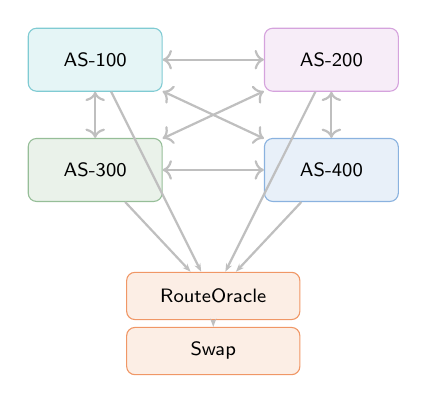
\begin{tikzpicture}[
  as/.style={draw,rounded corners=3pt,minimum width=1.7cm,minimum height=0.8cm,fill=#1!10,draw=#1!50,font=\sffamily\scriptsize,align=center},
  oracle/.style={draw,rounded corners=3pt,minimum width=2.2cm,minimum height=0.6cm,fill=eccaorange!10,draw=eccaorange!60,font=\sffamily\scriptsize,align=center},
  link/.style={-{Stealth[length=3pt]},thick,draw=gray!50}
]
\node[as=eccacyan]    (a) at (0,0)   {AS-100};
\node[as=eccamagenta] (b) at (3,0)   {AS-200};
\node[as=eccagreen]   (c) at (0,-1.4){AS-300};
\node[as=eccablue]    (d) at (3,-1.4){AS-400};
\node[oracle] (o) at (1.5,-3) {RouteOracle};
\node[oracle] (s) at (1.5,-3.7) {Swap};
\draw[link,<->] (a)--(b); \draw[link,<->] (a)--(c); \draw[link,<->] (a)--(d);
\draw[link,<->] (b)--(c); \draw[link,<->] (b)--(d); \draw[link,<->] (c)--(d);
\draw[link] (a) -- (o); \draw[link] (b) -- (o); \draw[link] (c) -- (o); \draw[link] (d) -- (o);
\draw[link,dashed] (o) -- (s);
\end{tikzpicture}
\caption{Experimental topology: four signed-BGP agents, all-to-all peering with injected latency, observed by a single \contractname{RouteOracle}/\contractname{Swap} pair in a shared namespace.}
\label{fig:topo}
\end{figure}

\subsection{Scripted scenarios}

The orchestrator (a cousin of the Playfair orchestrator) drives nine epochs of normal traffic, then triggers:

\begin{itemize}[leftmargin=*,itemsep=2pt]
  \item \textbf{Epoch 10 --- Origin hijack.} \code{as-300} announces a prefix owned by \code{as-100}. Two other agents detect, the first to submit proof claims the bounty.
  \item \textbf{Epoch 20 --- MOAS conflict.} \code{as-200} and \code{as-400} simultaneously announce the same prefix with different origins. Detection is symmetric; both agents race to file proof.
  \item \textbf{Epoch 30 --- Bad-signature flood.} \code{as-400} sends $10^{3}$ \code{SignedAdvertisement}s with random bytes for the signature. Verification cost is bounded; each failure mints one residue.
  \item \textbf{Epoch 35 --- Auto-pause trigger.} Sustained residue rate from \code{as-400} exceeds \code{autoPauseResidueRate}; the oracle pauses \code{as-400} automatically.
  \item \textbf{Epoch 40 --- Guardian intervention.} Two guardians invoke \code{emergencyPause} on \code{as-300} after a forensic dashboard review.
  \item \textbf{Epoch 45 --- Resume.} Three guardians sign a resume action for \code{as-300}; the pause clears.
\end{itemize}

\noindent Throughout, the existing Playfair \contractname{TripartiteGame} audit runs unchanged: routing-token consumption remains within per-region budgets.

\subsection{Pass criteria}

\begin{itemize}[leftmargin=*,itemsep=2pt]
  \item Every signed advertisement is verifiable from the public state of \code{StackIdentity}.
  \item Every detected residue is recorded on-chain with a valid proof.
  \item The first valid proof submitter receives the bounty exactly once.
  \item The auto-pause trigger fires within 2 epochs of threshold crossing.
  \item A 3-of-$N$ resume action takes effect in the next epoch.
  \item The \contractname{TripartiteGame} audit returns \code{fair} for all 50 epochs.
\end{itemize}

A self-contained HTML report (using the same generator pattern as Playfair) renders agent activity, residue timeline, guardian-action log, and pass/fail verdict.

\subsection{Reproducibility}

Bring-up is a single \code{bash tests/axonal-bgp/run.sh}, wrapping a Terraform module that mirrors Playfair's: \code{null\_resource} per phase, k3d cluster, image builds, image imports, manifest applies, orchestrator job, results extraction. CI nightly via \code{.github/workflows/axonal-bgp.yml}. The full source, Dockerfiles, and Terraform live under \code{tests/axonal-bgp/}.

% ============================================================
\section{Discussion}\label{sec:discussion}
% ============================================================

\subsection{Why not just sign with RPKI keys?}

RPKI keys are issued by RIRs to resource holders, not to autonomous agents. They are designed for static delegation, not for dynamic per-route signing. \axonal{} signatures are issued by \code{StackIdentity} NFTs, which are \emph{fluid}: an agent can be re-sleeved, migrated across regions, paused, resumed, or retired without losing identity continuity. Bridging the two is straightforward: a per-AS RPKI key can be embedded as a covenant in a \code{StackIdentity}'s metadata, anchoring agent identity to the existing trust hierarchy.

\subsection{Throughput}

Global BGP convergence events hit ${\sim}10^{5}$ UPDATEs/s. Per-message ed25519 verification on commodity hardware is ${\sim}50~\mu$s; a single core verifies ${\sim}2 \times 10^{4}$ UPDATEs/s. A four-core router agent meets the global ceiling. On-chain $\mathit{RouteTableRoot}$ commitments fire once per epoch (4~s), so chain throughput is not a bottleneck. The swap and oracle contracts each handle a single transaction per agent per detection event, well within Cortex EVM's capacity.

\subsection{Threat model}

\axonal{} provides defence against:
\begin{itemize}[leftmargin=*,itemsep=2pt]
  \item Origin hijack (RPKI parity).
  \item AS-path forgery (BGPsec parity, with smaller signatures).
  \item Coordinated misbehaviour (residue economy makes it costly).
  \item Routing-table tampering (per-epoch on-chain commitments).
\end{itemize}

\noindent It does \emph{not} provide defence against:
\begin{itemize}[leftmargin=*,itemsep=2pt]
  \item Data-plane attacks (a peer that signs correct routes but drops packets).
  \item Compromised guardians colluding to keep a malicious agent unpaused.
  \item Catastrophic Cortex chain compromise (would invalidate the swap, but the routing layer continues to function on signature checks alone).
\end{itemize}

\subsection{Limitations}

The experimental demo runs four agents in a single cluster. Inter-cluster federation, multi-region oracle redundancy, and long-tail RPKI bridging are out of scope for v0.1. The bounty values in the residue catalogue are illustrative; calibration against real-world incident data is future work. The choice of CBOR over BGP \code{OPTIONAL\_TRANSITIVE} attribute encoding optimises for tooling familiarity; a wire-compatible BGP-attribute encoding is straightforward but unimplemented.

\subsection{Deployment paths}

Three plausible adoption paths:
\begin{enumerate}[leftmargin=*,itemsep=2pt]
  \item \textbf{Greenfield mesh.} Operators of new networks (research, DePIN, mesh) deploy \axonal{} alongside conventional BGP and weight signed routes higher.
  \item \textbf{Sidecar deployment.} Existing operators run the router agent as a passive observer that emits residues but does not yet alter forwarding decisions.
  \item \textbf{Selective trust.} A consortium of cooperating ASes peers exclusively over \axonal{} and treats the oracle as authoritative for that subgraph.
\end{enumerate}

% ============================================================
\section{Conclusion}\label{sec:conclusion}
% ============================================================

Inter-domain routing and distributed cognition share a deep structural similarity: both are about \emph{attesting state} across a federation of independently-administered systems. \ecca{}'s substrate---portable identity, atomic cross-shard finality, residue-funded self-healing---is well-suited to this problem. \axonal{} shows that with two new smart contracts (a one-way \contractname{ResidueToRoutingSwap} and a multisig-gated \contractname{RouteOracle}) and one new microservice, an experimental routing protocol can be assembled that combines cryptographic per-route signatures, an in-band economic loop for misbehaviour detection, and a human-in-the-loop emergency stop. The reproducible k3d demonstration shows the protocol surviving four scripted incident classes within the same fairness audit that governs the rest of the \ecca{} system.

Future work includes wire-compatible BGP encoding, integration with live RPKI, an adversarial benchmark against historical incidents, and economic calibration of bounty parameters from operational data.

\balance

\bibliographystyle{plain}
\bibliography{references}

\end{document}
